\documentclass{article}
\usepackage{graphicx} % Required for inserting images
\usepackage{amsmath}
\usepackage[backend=biber]{biblatex}
\usepackage{hyperref}

\addbibresource{references.bib}

\title{5511 hw2}
\author{Tony Siu}
\date{September 2024}

\begin{document}
\maketitle
\section{Derivation of average cost for binary search for sorted array \cite{Knuth1998}\cite{chatgpt2024}}

\hspace{\parindent}The average number of steps in a binary search is influenced by the likelihood of targeting each specific element. There's a distinction between the number of steps needed in searches that find an element (successful searches) and those that do not (unsuccessful searches). For successful searches, it is presumed that every element has an equal chance of being the target. In the case of unsuccessful searches, it is assumed that every possible unsuccessful search between elements, as well as numeric values beyond the available array has an equal chance of being the search target. Thus, the average iterations needed for successful searches is calculated by the total iterations taken to locate each element once, divided by n, the total number of elements. Conversely, the average iterations for unsuccessful searches is determined by the total iterations to check each possible interval once, divided by n + 1, the total number of these gaps.

\subsection{Successful Search}

\hspace{\parindent}I would like to represent the binary search algorithm for a sorted array as a binary tree representation. In a binary tree model, finding a target within a sorted array via binary search can be depicted as traveling along a route from the tree's root down to the designated node, known as an internal path. This path's length, determined by the count of edges it crosses, directly impacts the number of iterations needed to complete the search — specifically, the path length plus one, accounting for the initial step in the search process. The total length of all such paths within the tree, termed the internal path length and symbolized as $I(n)$, reflects the cumulative steps needed to individually locate each of the nn elements, where nn is the total number of nodes (or elements) in the array. Consequently, the average iterations for a successful search are calculated using the formula $T(n) = 1 + \frac{I(n)}{n}$, incorporating an extra iteration to include the starting point. 

% \newline
% \hfill 
\break
% \vspace{5mm}
Given binary search's status as the most efficient comparative search technique, determining this average effectively boils down to calculating the shortest possible internal path lengths across all conceivable binary trees containing nn nodes. This minimal length is given by:

$$I(n) = \sum_{k=1}^n \left \lfloor {log_2 (k)}\right \rfloor$$

For instance, consider an array with 7 elements. Here, locating the root element takes a single iteration, finding either of the next two elements requires two iterations each, and identifying any of the following four elements demands three iterations apiece. Thus, the total internal path length for this array configuration is:

$$\sum_{k=1}^{7} \left \lfloor {log_2 (k)}\right \rfloor = 0 + 2(1) + 4(2) = 2 + 8 = 10$$

The average number of iterations would be $1 + \frac{10}{7} = 2\frac{3}{7}$ based on the equation for the average case. The sum for $I(n)$ can be simplified to:

$$I(n) = \sum_{k=1}^n \left \lfloor {log_2 (k)}\right \rfloor = (n + 1) \left \lfloor {log_2 (n + 1)}\right \rfloor - 2^{\left \lfloor {log_2 (n + 1)}\right \rfloor + 1} + 2$$

Substituting the equation for $I(n)$ into the equation for $T(n)$:

$$T(n) = 1 + \frac{(n + 1)\left \lfloor {log_2 (n + 1)}\right \rfloor - 2^{\left \lfloor {log_2 (n + 1)}\right \rfloor + 1} + 2}{n} = \left \lfloor {log_2 (n)}\right \rfloor  + 1  - \frac{(2^{\left \lfloor {log_2 (n)}\right \rfloor  + 1} - \left \lfloor {log_2 (n)}\right \rfloor  - 2)}{n}$$

For integer n, this is equivalent to the equation for the average case on a successful search specified above.

\subsection{Unsuccessful Search}

\hspace{\parindent}

When a binary search does not find the target value in an array, you can think of this process as navigating through a specially designed binary tree that includes additional "external" nodes. These external nodes fill every possible gap where an element could be but isn't, ensuring every potential position has a corresponding node. Internal nodes are the nodes the represent the actual elements in the array. External nodes are added to account for every position where there could have been and element but isn't, including spaces before the first element and after the last one.
\newline

In unsuccessful searches, we trace a path from the root of the tree (the beginning) to one of these external nodes. The sum of the lengths of all these paths is known as the external path length, denoted $E(n)$.

To compute the average number of steps for an unsuccessful search, we use the external path length divided by $n+1$, where $n$ is the number of actual elements in the array. This division by $n+1$ accounts for all the gaps between elements and the spaces outside the boundaries of the array. The calculation of $E(n)$ includes an internal path length $I(n)$ which sums up the number of steps to reach each element if it were the target of the search. There is an additional 2 steps for every element because in this expanded tree each internal nodes has 2 children. The formula for the external path length thus combines these values as $E(n) = I(n) + 2n$. Using this formula, the average number of iterations required for unsuccessful searches is calculated as $T^\prime(n) = \frac{E(n)}{n + 1}$. This way, the average number of steps for unsuccessful searches evaluates how long it would take to reach every potential placements where the target isn't and averages that over all those placements. Substituting the equation for $I(n)$:

$$E(n) = I(n) + 2n = [(n + 1)\left \lfloor {log_2 (n + 1)}\right \rfloor - 2^{\left \lfloor {log_2 (n + 1)}\right \rfloor + 1} + 2] + 2n = (n + 1)(\left \lfloor {log_2 (n)}\right \rfloor + 2) - 2^{\left \lfloor {log_2 (n)}\right \rfloor + 1}$$

Substituting the equation for $E (n)$  into the equation for $T^\prime(n)$, the average case for unsuccessful searches can be determined:

$$T^\prime(n) = \frac{(n + 1)(\left \lfloor {log_2 (n)}\right \rfloor + 2) - 2^{\left \lfloor {log_2 (n)}\right \rfloor + 1}}{n + 1} = \left \lfloor {log_2 (n)}\right \rfloor + 2 - \frac{2^{\left \lfloor {log_2 (n)}\right \rfloor + 1}}{n + 1}$$

\section{Case studies of Binary Search given assumptions\cite{chatgpt2024}}
\subsection{Assumption 1}

\hspace{\parindent}\emph{The value to be searched appears at any position in the array with the same probability, which is also the probability that there is no such a value in the array.}
\break
In this case, the probability that the value is at any specific position is pp, and the probability that the value is not in the array is also pp. Since there are n positions plus the possibility of the value not being in the array, the total probabilities sum up to $(n + 1)p = 1$ Thus, $p = \frac{1}{n + 1}$.

\begin{itemize}
    \item Probability of successful search: $P_{success} = n \times p = \frac{n}{n + 1}$
     \item Probability of unsuccessful search: $P_{failure} = p = \frac{1}{n + 1}$
\end{itemize}

The average number of iterations for a successful search ($T_g$) and an unsuccessful search ($T_u$) can be approximated as:

\begin{itemize}
    \item Successful search $T_s \approx log_2n$
     \item Unsuccessful search $T_s \approx log_2n + 1$
\end{itemize}

Under Assumption 1:

\begin{flalign}
    \begin{aligned}
    Expected Iterations_1 = & P_{success} \times T_{s} + P_{failure} \times T_{u} \\
    & = (\frac{n}{n + 1} \times log_2n) + (\frac{1}{n + 1} \times (log_2n + 1))\\
    & = log_2n(\frac{n}{n + 1} + \frac{1}{n + 1}) + \frac{1}{n + 1}\\
    & = log_2n + \frac{1}{n + 1} 
    \end{aligned}  
\end{flalign}
  





\subsection{Assumption 2}

\hspace{\parindent}\emph{The probability of the value to be in the array is the same as the probability of the opposite case (the value is not there), and when it is in the array the probability for it to appear in any position is the same.}
\newline

Here, the probability that the value is in the array is 0.50.5, and if it is, the probability that it's at any specific position is 1n $\frac{1}{n}$. Therefore, the total probability that the value is at a specific position is $0.5 \times \frac{1}{n} = \frac{1}{2n}$. 

\begin{itemize}
    \item Probability of successful search: $P_{success} = 0.5, P_{success_i} = \frac{\frac{1}{2}}{n}$ 
     \item Probability of unsuccessful search: $P_{failure} = 0.5$
\end{itemize}


Under Assumption 2:
\begin{flalign}
    \begin{aligned}
    Expected Iterations_2 = & P_{success} \times T_{s} + P_{failure} \times T_{u} \\
    & = (0.5 \times log_2n) + (0.5 \times (log_2n + 1))\\
    & = log_2n + 0.5
    \end{aligned}  
\end{flalign}





\subsection{Comparison}

\hspace{\parindent}The average running time (in terms of iterations) under Assumption 2 is higher than under Assumption 1. This is because under Assumption 2, there's a higher probability of an unsuccessful search (50\% vs. a much smaller $\frac{1}{n + 1}$ in Assumption 1), and unsuccessful searches require more iterations on average. Therefore, the algorithm does not have the same average running time in both situations, and the average running time is higher under Assumption 2.



\section{Why average cost and worst cost of binary search is both $O(log n)$\cite{chatgpt2024}}

\hspace{\parindent}The average cost and worst-case cost of the binary search algorithm are both $O(log⁡n)$ because they both grow logarithmically with the size of the input n. The difference is a constant or a lower-order term, which doesn't affect the Big O classification.

$$T_{worst}(n) = \left \lceil {log_2n}\right \rceil$$
$$T_{average}(n)  \approx log_2n + c$$


\subsection{Binary Search Complexity}

\subsection{Worst-Case Cost}
\begin{itemize}
    \item \textbf{Scenario:} The worst-case occurs when the target value is not in the array or is located in such a way that requires the maximum number of iterations to find.
    \item {\textbf{Iterations Needed:} The maximum number of iterations (comparisons) in binary search is $\left \lceil {log_2 (n)}\right \rceil$, where $\left \lceil {x}\right \rceil$, denotes the smallest integer greater than or equal to x.}
    \item {\textbf{Explanation:} Each iteration divides the search interval in half. Therefore, after $log⁡_2n$ iterations, the interval reduces to a single element.}
    \item \textbf{Result:} The worst-case cost is proportional to log⁡n.
\end{itemize}


\subsubsection{Average-Case Cost}
\begin{itemize}
    \item \textbf{Scenario:} Calculated under the assumption that each element (and interval between elements for unsuccessful searches) is equally likely to be searched.
    \item \textbf{Iterations Needed:} As derived in the simplified equations, the average number of iterations for successful and unsuccessful searches are both approximately $log⁡_2n$, but slightly less than the worst-case cost.
    \item \textbf{Explanation:} Each iteration divides the search interval in half. Therefore, after $log⁡_2n$ iterations, the interval reduces to a single element.
    \item \textbf{Result:} The average-case cost is also proportional to $log⁡_n$.
\end{itemize}


\section{Estimate average cost with program}
Here is the \href{https://github.com/Tony363/5511/blob/main/hw2/binary_search.py}{code link} to my implementation.
\newline

Here, I estimated the average number of iterations required by the binary search algorithm for arrays of different sizes. I generate sorted arrays of various, perform large number of searches, both successful and unsuccessful search on each array size and record the number of iterations. The average number of iterations for successful and unsuccessful searches is aggregated. I used Assumption 2 from the earlier discussion:
\begin{itemize}
    \item Probability of value being in the array : 50\%
    \item When the value is in the array: It is equally likely to be any of the elements
    \item When the value is not in the array: it is equally liekly to be any value not in the array.
\end{itemize}

The assumption provides a balanced mix of successful and unsuccessful searches suitable for empirical analysis.
\begin{figure}
\centering
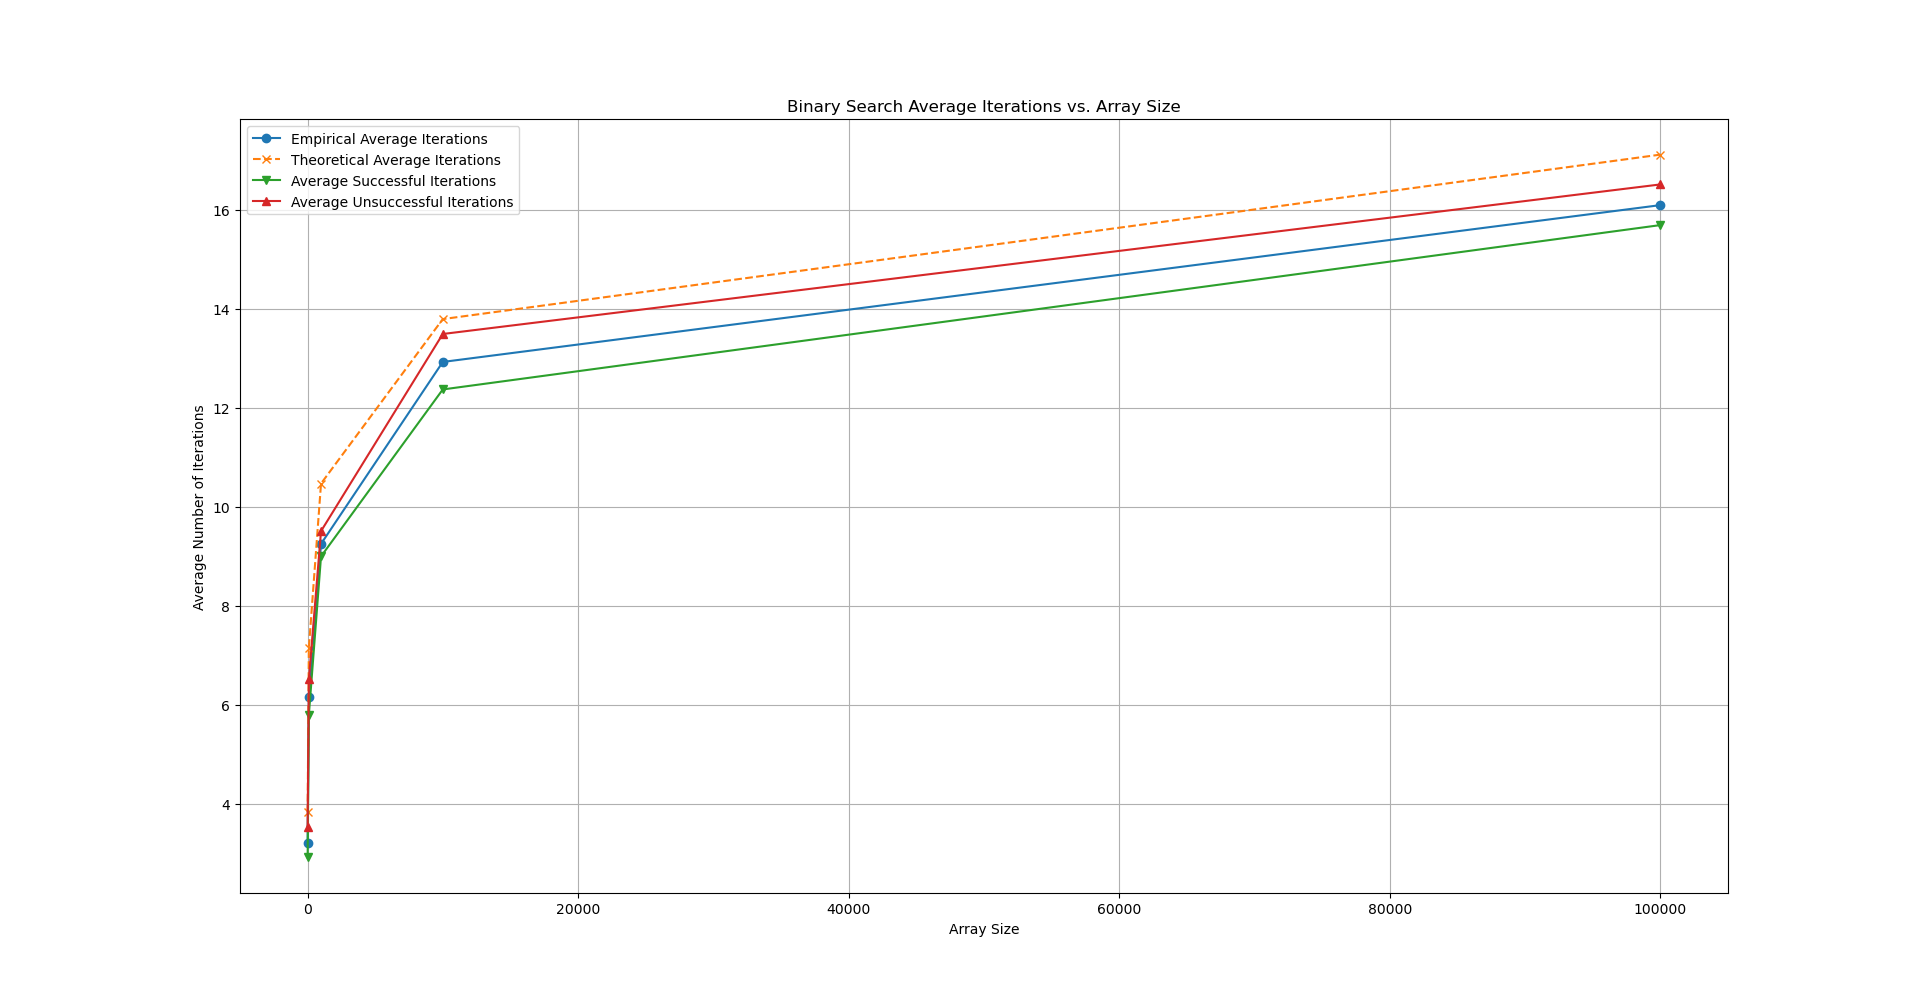
\includegraphics[scale=0.25]{not_log.png}
\end{figure}

\begin{figure}
\centering
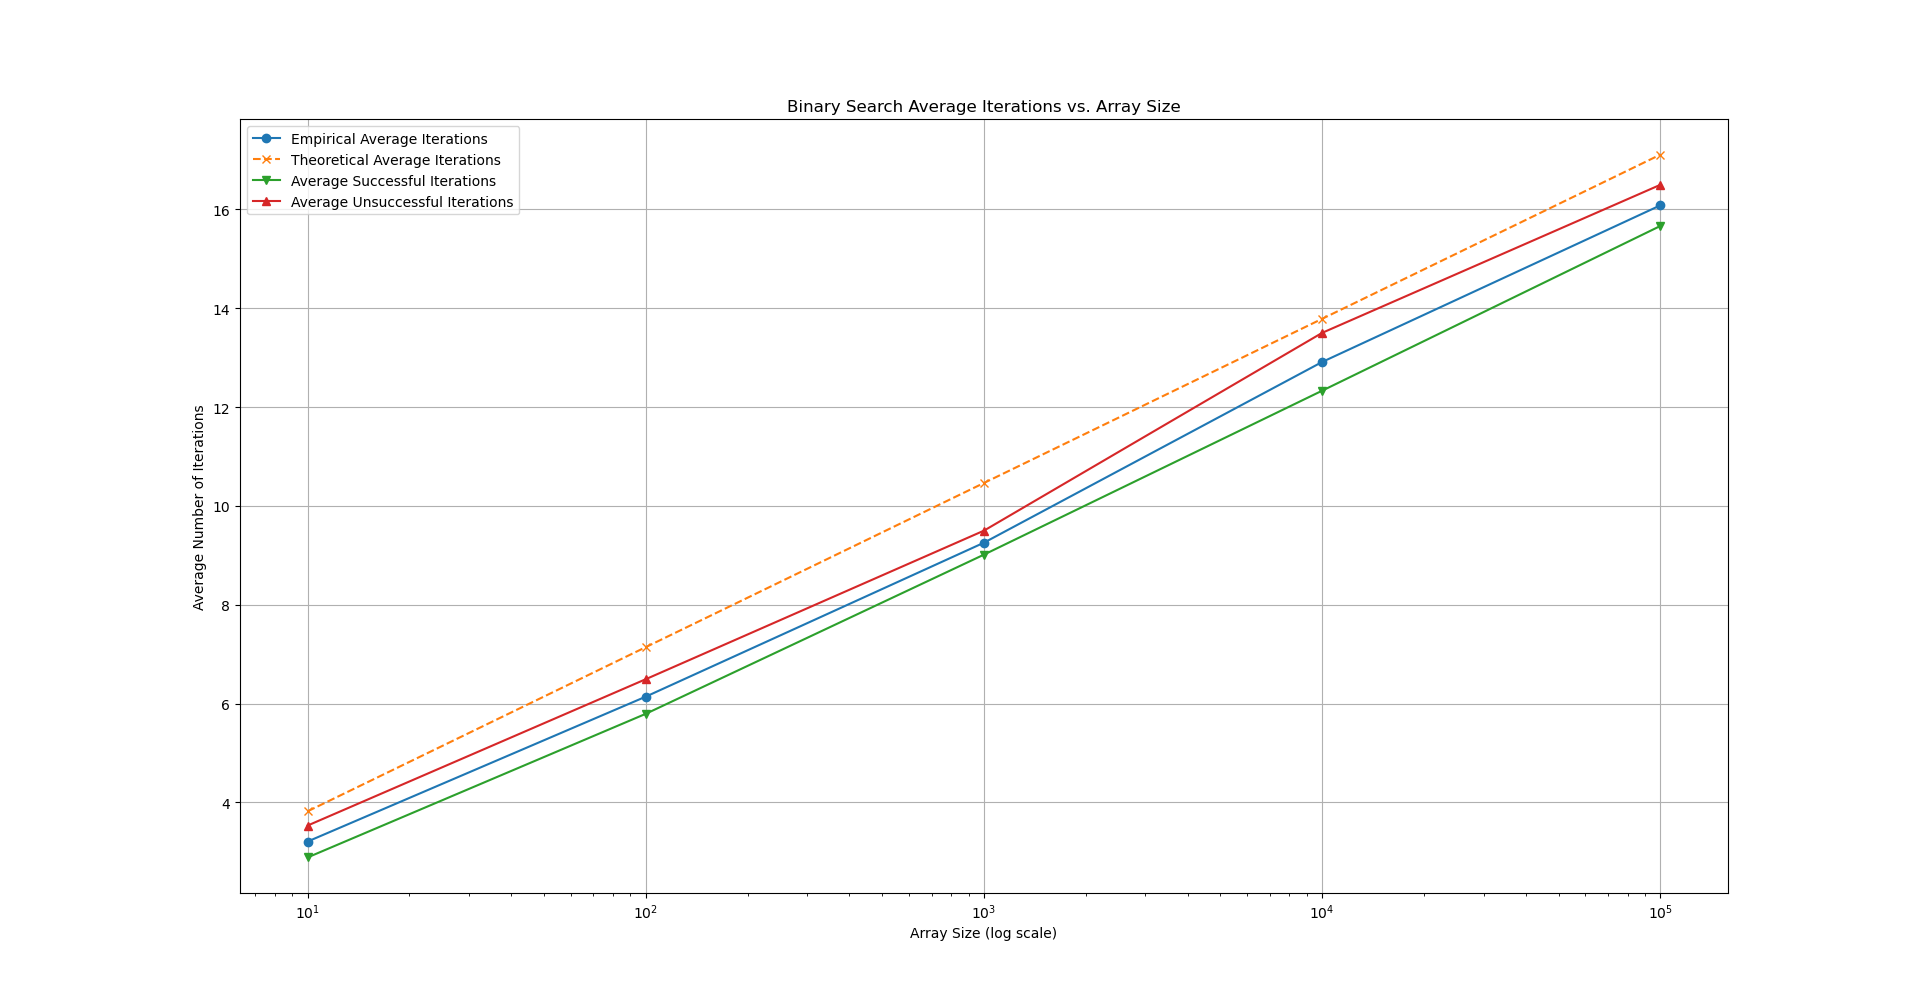
\includegraphics[scale=0.25]{log.png}
\end{figure}



\subsection{Program Outputs}
\begin{itemize}
  \item \textbf{Array Size: 10}
  \item Average Total Iterations: 3.2100
  \item Average Successful Iterations: 2.8883
  \item Average Unsuccessful Iterations: 3.5336
  \item Theoretical Average Iterations: 3.8219    
\end{itemize}


\begin{itemize}
    \item \textbf{Array Size: 100}
    \item Average Total Iterations: 6.1420
    \item Average Successful Iterations: 5.7947
    \item Average Unsuccessful Iterations: 6.4952
    \item Theoretical Average Iterations: 7.1439
\end{itemize}



\begin{itemize}
    \item \textbf{Array Size: 1000}
    \item Average Total Iterations: 9.2573
    \item Average Unsuccessful Iterations: 9.5011
    \item   Theoretical Average Iterations: 10.4658
\end{itemize}
  
\begin{itemize}
    \item \textbf{Array Size: 10000}

    \item Average Total Iterations: 12.9140
    \item  Average Successful Iterations: 12.3330
    \item Average Unsuccessful Iterations: 13.5034
    \item   Theoretical Average Iterations: 13.7877
\end{itemize}


\begin{itemize}
    \item \textbf{Array Size: 10000}
    \item Average Total Iterations: 16.0835
    \item Average Successful Iterations: 15.6660
    \item Average Unsuccessful Iterations: 16.4990
    \item   Theoretical Average Iterations: 17.1096
\end{itemize}
  
\subsection{Discussion}

\hspace{\parindent}The emperical average iterations are slightly lower than the theoretical values. The discrepancy decreases as the array size increases. Unsuccessful searches generally require slightly more iterations than successful searches, aligning with the theoretical understanding. The difference between successful and unsuccessful searches becomes negligible as the array size increases. The average number of iterations increases logarithmically with the array size. This confirms the $O(log⁡_n)$ time complexity of binary search.
\newline

The theoretical expected iterations is $log_2n + 0.5$. For large n, the empirical average iterations apporach $log_2n$ rather than $log_2n + 0.5$. The slight difference may be due to the way iterations are counted in the code and hte probabilistic nature of the simulations.
\newline

In conclusion, The simulation confirms that the average number of iterations required by binary search grows logarithmically with the array size. The empirical results are consistent with the theoretical analysis, showing that both successful and unsuccessful searches have an average cost of $O(log⁡_n)$. In practice, binary search is highly efficient for large datasets, as the number of iterations increases very slowly with the size of the array.

\printbibliography

\end{document}
